\exercise

Given the sequence of strings $S = [ \text{\tt cat}, \text{\tt abi}, \text{\tt
cast}, \text{\tt car}, \text{\tt at} ]$,
%
\begin{enumerate}
  \item Insert them in a TST in that order.

  \item Given a set of $n$ strings of length $L$ over an alphabet $A$, propose and
  discuss a variant of Multi-key quicksort that partitions those strings over
  the recursive calls according to a group of $g$ characters instead of a single
  one, and analyze the time complexity of the proposed algorithm as a function
  of $g$ (i.e. when $g$ grows more than the word-memory size).

\end{enumerate}

\solution

\begin{enumerate}

  \item \autoref{fig:TST} shows the changing of the TST's topology after the
  insertion of the strings contained in $S$.

  \item \autoref{alg:mkqs} shows the revisited version of the Multi-key
  Quicksort using grouped comparisons of $g$ characters ($<_g$, $=_g$, and
  $>_g$). As in classical Multi-key Quicksort, each string will end up either in
  $R_< \cup R_>$ or in $R_=$. In the first case, the string will end up in a
  subset of $R$, with $|R_< \cup R_>| \le \alpha n$ and $\alpha < 1$. In the
  other case the set might remain the same (all the strings begin with the same
  group of $g$ characters), but the $i$ will be increased by $g$. Both cases
  will cost $O(1)$ time if $g$ characters occupy less or equal than the word
  size $w$, otherwise they will cost in the worst case $O\big(\left\lceil
  \frac{g}{w} \right\rceil \big)$ single character comparisons. The number of
  $g$-comparisons for each string is $O\Big(\left\lceil \frac{|s|}{g}
  \right\rceil + \log n \Big)$. Multiplying for the number of strings in $R$ we
  obtain $O\Big(\left\lceil \frac{|s|}{g} \right\rceil + n\log n \Big) \approx
  O\big(\frac{N}{g} + n\log n \big)$. When $g > w$ we have $O\big(\left\lceil
  \frac{g}{w} \right\rceil \cdot \frac{N}{g} + \log n \big) \approx
  O\big(\frac{N}{w} + \log n \big)$, meaning that we obtain no benefit from
  increasing $g$ more than the word size. We should also notice that creating
  groups of characters we are implicitly resizing the alphabet from $O(\sigma)$
  to $O(\sigma^g)$. This will cause the revisited Multi-key Quicksort to create
  singletons when partitioning $R_=$ on small datasets, thus increasing the
  number of recursive iterations on $R_< \cup R_>$.

\end{enumerate}
%
\begin{figure}[ht]
  \centering
  \tikzstyle{level 1}=[level distance=1.5cm, sibling distance=1.5cm]
  \tikzstyle{level 2}=[level distance=1.5cm, sibling distance=1.5cm]
  \tikzstyle{level 3}=[level distance=1.5cm, sibling distance=1.5cm]

  \hspace{-0.175\linewidth}%
  \begin{subfigure}[b]{0.25\linewidth}
    \begin{subfigure}[t]{\columnwidth}
      \centering
      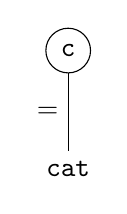
\begin{tikzpicture}[grow=down]
      \node[draw,fill=white, circle] {\tt c}
          child {
              node[draw=none] {\tt cat}
                  edge from parent[-] node[left] {=}
          };
      \end{tikzpicture}
      \caption{}
    \end{subfigure} \\\vspace{3em}

    \begin{subfigure}[t]{\columnwidth}
      \centering
      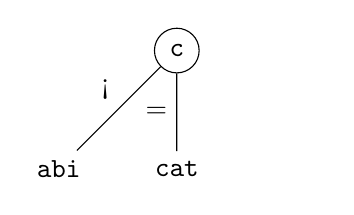
\begin{tikzpicture}[grow=down]
      \node[draw,fill=white, circle] {\tt c}
          child {
              node[draw=none] {\tt abi}
                  edge from parent[-] node[above left] {<}
          }
          child {
              node[draw=none] {\tt cat}
                  edge from parent[-] node[left] {=}
          }
          child {
              node[draw=none] {\phantom{\tt cat}}
                edge from parent[draw=none]
          };
      \end{tikzpicture}
      \caption{}
    \end{subfigure}
  \end{subfigure}\hspace{-0.05\linewidth}
  \begin{subfigure}[t]{0.25\columnwidth}
    \centering
    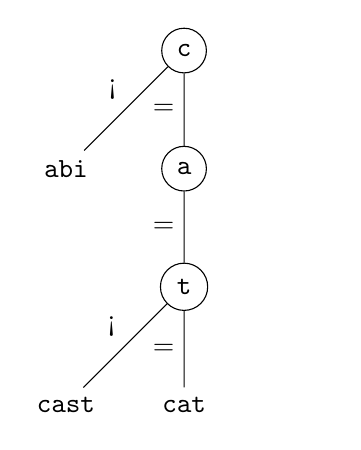
\begin{tikzpicture}[grow=down]
    \node[draw,fill=white, circle] {\tt c}
        child {
            node[draw=none] {\tt abi}
                edge from parent[-] node[above left] {<}
        }
        child {
            node[draw, circle] {\tt a}
                child {
                    node[draw, circle] {\tt t}
                        child {
                          node[draw=none] {\tt cast}
                              edge from parent[-] node[above left] {<}
                        }
                        child {
                          node[draw=none] {\tt cat}
                              edge from parent[-] node[left] {=}
                        }
                        child {
                          node[draw=none] {}
                              edge from parent[draw=none]
                        }
                        edge from parent[-] node[left] {=}
                }
                edge from parent[-] node[left] {=}
        }
        child {
            node[draw=none] {\phantom{\tt cat}}
              edge from parent[draw=none]
        };
    \end{tikzpicture}
    \caption{}
  \end{subfigure}
  \hspace{-0.05\linewidth}
  \begin{subfigure}[t]{0.23\columnwidth}
    \centering
    \begin{tikzpicture}[grow=down]
    \node[draw,fill=white, circle] {\tt c}
        child {
            node[draw=none] {\tt abi}
                edge from parent[-] node[above left] {<}
        }
        child {
            node[draw, circle] {\tt a}
                child {
                    node[draw, circle] {\tt t}
                        child {
                            node[draw, circle] {\tt s}
                                child {
                                  node[draw=none] {\tt car}
                                      edge from parent[-] node[above left] {<}
                                }
                                child {
                                  node[draw=none] {\tt cast}
                                      edge from parent[-] node[left] {=}
                                }
                                child {
                                  node[draw=none] {}
                                      edge from parent[draw=none]
                                }
                              edge from parent[-] node[above left] {<}
                        }
                        child {
                          node[draw=none] {\tt cat}
                              edge from parent[-] node[left] {=}
                        }
                        child {
                          node[draw=none] {}
                              edge from parent[draw=none]
                        }
                        edge from parent[-] node[left] {=}
                }
                edge from parent[-] node[left] {=}
        }
        child {
            node[draw=none] {}
              edge from parent[draw=none]
        };
    \end{tikzpicture}
    \caption{}
  \end{subfigure}
  \hspace{-0.05\linewidth}
  \begin{subfigure}[t]{0.5\columnwidth}
    \centering
    \begin{tikzpicture}[grow=down]
    \node[draw,fill=white, circle] {\tt c}
        child[sibling distance=4.5cm] {
            node[draw, circle] {\tt a}
            child {
              node[draw, circle] {\tt b}
              child {
                node[draw=none] {}
                    edge from parent[draw=none]
              }
              child {
                node[draw=none] {\tt abi}
                    edge from parent[-] node[left] {=}
              }
              child {
                node[draw=none] {\tt at}
                    edge from parent[-] node[above right] {>}
              }
              edge from parent[-] node[left] {=}
            }
            edge from parent[-] node[above left] {<}
        }
        child {
            node[draw, circle] {\tt a}
                child {
                    node[draw, circle] {\tt t}
                        child {
                            node[draw, circle] {\tt s}
                                child {
                                  node[draw=none] {\tt car}
                                      edge from parent[-] node[above left] {<}
                                }
                                child {
                                  node[draw=none] {\tt cast}
                                      edge from parent[-] node[left] {=}
                                }
                                child {
                                  node[draw=none] {}
                                      edge from parent[draw=none]
                                }
                              edge from parent[-] node[above left] {<}
                        }
                        child {
                          node[draw=none] {\tt cat}
                              edge from parent[-] node[left] {=}
                        }
                        child {
                          node[draw=none] {}
                              edge from parent[draw=none]
                        }
                        edge from parent[-] node[left] {=}
                }
                edge from parent[-] node[left] {=}
        }
        child {
            node[draw=none] {}
              edge from parent[draw=none]
        };
    \end{tikzpicture}
    \caption{}
  \end{subfigure}
  \hspace{-0.25\linewidth}
  \caption{Topology of the TST after the insertion of the strings in $S$.}
  \label{fig:TST}
\end{figure}
%
\begin{algorithm}[hb]
\caption{Revisited Multi-key Quicksort}\label{alg:mkqs}
\begin{algorithmic}[1]
  \Function{RevMultiKeyQS}{$R$, $i$, $g$}
    \If{$|R| \le 1$}
      \State \Return $R$
    \EndIf
    \State Choose a pivot $p \in R$
    \State $R_< = \left\{ s \in R \mid s[i, i+g] <_g p[i, i+g]  \right\}$
    \State $R_= = \left\{ s \in R \mid s[i, i+g] =_g p[i, i+g]  \right\}$
    \State $R_> = \left\{ s \in R \mid s[i, i+g] >_g p[i, i+g]  \right\}$
    \State $A =$ \Call{RevMultiKeyQS}{$R_<$, $i$, $g$}
    \State $B =$ \Call{RevMultiKeyQS}{$R_=$, $i+g$, $g$}
    \State $C =$ \Call{RevMultiKeyQS}{$R_>$, $i$, $g$}
    \State \Return $A \oplus B \oplus C$
  \EndFunction
\end{algorithmic}
\end{algorithm}
